\chapter{Results and Discussion}\label{chapter:results}
This chapter includes presentation and analysis of the results obtained in this thesis. Section \ref{section:parameter settings} presents results from testing different parameter settings for the genetic algorithm, and briefly discusses each results. Section \ref{section:results} presents the main results obtained when running the different population distributed genetic algorithms. Section \ref{section:discussion} contains a discussion and comparison of the results obtained in section \ref{section:results}.


\section{Parameter settings}\label{section:parameter settings}
Parameter settings are crucial for obtaining good results with the genetic algorithm, therefore, this whole section is devoted to the process. Simulations were run to find the best adult selection method, parent selection method, crossover method, crossover rate and mutation rate for the given problem. Even though it would take much less time and effort to test these values on a toy problem, such as One Max, the decision was made to test them on the real problem. The reason for this is that it is not necessarily true that the parameter values most fit to solve the One Max problem is the same as those most fit to solve the wind farm layout optimization problem. In the wind farm layout optimization problem the relative positions of the turbines are extremely important, this property distinguishes wind farm layout optimization from other problems and could mean that it needs different parameter values than a toy problem with different properties.\\

\noindent It is important to note that even though effort was made to find the right parameter values for the genetic algorithm, it is impossible to obtain the optimal ones. Just imagine trying to test every single value of the continuous parameter crossover rate, just that would be impossible! Therefore, the values that are tested for each parameter are based on the authors previous knowledge and experience with genetic algorithms. \\

\noindent For each simulation presented in this section one parameter were optimized while the others were kept fixed with the values shown in table \ref{table:fixed settings}. The parameters in the table are common for all the genetic algorithm models implemented in this thesis, however, they are only optimized when run on the Master/Slave model. Ideally, they should be optimized for all of the models, but that would not be possible within the time frame of this thesis.\\ 

\begin{table}[h!]
\centering
\caption{Values that were kept fixed while one by one were optimized to find the correct settings for the find farm layout optimization problem.}
\label{table:fixed settings}
\begin{tabular}{l|l}
\textbf{Parameter} & \textbf{Value} \\ 
\hline 
Wind scenario & 00.xml \\ 
Evaluator & KusiakLayoutEvaluator \\ 
Population size & 100 \\  
Generations & 100 \\ 
Elitism & true \\  
Flip mutation rate & 0.01 \\ 
Inversion mutation rate & 0.0 \\ 
Interchange mutation rate & 0.0 \\ 
Parent selection & Tournament selection \\ 
Tournament size & 5\% of population size \\ 
Epsilon & 0.1 \\  
Crossover method & Uniform crossover \\ 
Crossover rate & 0.9 \\ 
\end{tabular} 
\end{table}

\noindent As can be seen in table \ref{table:fixed settings}, other parameters such as wind scenario, population size, number of generations, whether elitism should be used and mutation rate for interchange mutation and inversion mutation could also be optimized. However, as explained above, the time frame of this thesis prevented the author from running these simulations. These variables are therefore set using the authors previous experience with genetic algorithms. Testing different parameter values on a single wind scenario might lead to values that are tailored for the given scenario and that are not as well suited for some of the other scenarios. However, the author does not believe this to be crucial for the final results. Population size is a value that heavily influence the performance of the genetic algorithm, because greater population size increase the probability of finding the global best solution. When testing parameter values, the population size was kept at 100 for two reasons: First, a population size of 100 is large enough so that many different solutions can be explored. Second, when the population size was kept at 100, the adult selection mechanism overproduction would require 200 evaluations each generation. This doubles the evaluation time, the step that is already the bottleneck of the algorithm. Elitism was set to true for every run, meaning that the best individual of each generation will survive. This decision is based on the authors previous experience with genetic algorithms, where experiments has shown that elitism leads to better results because the best individual is not lost due to coincidences. Three different mutation methods were implemented, but experiments were only run to find the optimal value for the flip mutation rate. Usually, flip mutation is the only mutation method used with genetic algorithms and it is therefore also used as the main mutation method in this thesis. Inversion mutation and interchange mutation will also be used, but they will be assigned low enough probabilities so that they will not make trouble, but hopefully, lead to occasional, rare jumps from one part of the solution space to another so that the population do not get stuck in a local minima.\\

\noindent In summary, the sub-sections below contain simulations run to find the parameter values most suited for the wind farm layout optimization problem. The resulting parameter values will be used for all 4 genetic algorithm models in section \ref{section:results}. In order to get trustworthy results, each simulation is run 10 times and the plots shown in the subsequent sub-sections are averaged over these 10 simulations. Even though all the models are implemented to run in parallel it takes half a day to run one simulation on an 8 core computer, this is the reason why only the most crucial parameters are optimized and why they are only optimized on the Master/Slave model even though they will be used by the other models as well.\\

\subsection{Adult Selection}
Figure \ref{plot:adult selection methods} shows the results of running the genetic algorithm with the three different adult selection methods. Sub-figure \ref{plot:full generational replacement}, \ref{plot:generational mixing}, and \ref{plot:overproduction} shows the results for full generational replacement, generational mixing and overproduction respectively. \\

\noindent The results show that full generational replacement ends up with worse fitness than both generational mixing and overproduction, and that overproduction is the method that is able to achieve the best fitness of the three. These results agrees with the authors previous experience. Note that with generational mixing, only the solutions from the new child population that are better than those in the previous adult population are allowed to enter the adult pool. This means that from one generation to another the average fitness of the new adult population can never be worse than the average fitness of the previous adult population. If every new solution generated is worse than those from the previous generation, the previous generation is given another attempt to reproduce and the fitness from one generation to another is left unchanged. However, if one or more of the new solutions are better than those in the previous generation they will be allowed into the adult pool, and the new adult pool will have better fitness than the previous. Full generational replacement does not take this greedy approach. It replaces the entire previous adult population, even though that might lead to worse average fitness from one generation to another. This does not however mean that full generational replacement always obtains worse final results compared to generational mixing. On this problem however, it seems like the greedy approach taken by generational mixing works well for wind farm layout optimization. Overproduction will, as full generational replacement, replace the entire previous adult pool with new individuals. However, with overproduction, the probability that the new adult population will have better average fitness is much higher since it has twice as many children to choose from. This means that even though it is not guaranteed, it is likely that the new adult population will have higher fitness than the previous one. The results show that overproduction is the most suitable adult selection method for the wind farm layout optimization problem.\\

\begin{figure}[h!]
    \centering
    \begin{subfigure}[b]{0.31\textwidth}
        \includegraphics[width=\textwidth]{images/plots/"adult selection"/"full generational replacement"}
        \caption{}
        \hfill
        \label{plot:full generational replacement}
    \end{subfigure}
    ~
    \begin{subfigure}[b]{0.31\textwidth}
        \includegraphics[width=\textwidth]{images/plots/"adult selection"/"generational mixing"}
        \caption{}
        \hfill
        \label{plot:generational mixing}
    \end{subfigure}
    ~
    \begin{subfigure}[b]{0.31\textwidth}
        \includegraphics[width=\textwidth]{images/plots/"adult selection"/"overproduction"}
        \caption{}
        \hfill
        \label{plot:overproduction}
    \end{subfigure}
    \caption{Adult selection methods: (a) Full generational replacement, (b) generational mixing and (c) overproduction. Each plot shows the averaged results obtained when running each scenario 10 times.}
    \label{plot:adult selection methods}
\end{figure}

\subsection{Parent Selection}
Figure \ref{plot:parent selection} shows the results for running the genetic algorithm with parent selection methods roulette wheel in sub-figure \ref{plot:roulette wheel}, and tournament selection in sub-figures \ref{plot:tournament size 5} - \ref{plot:tournament size 25}. Tournament selection is run with five different values for the variable \textit{tournament size}. Clearly, roulette wheel do not work well for this problem. Roulette wheel assigns each individual a probability of being selected proportional to its fitness, and since there is not a large difference in fitness of the different individuals the selection becomes almost random. With tournament selection on the other hand, this problem is taken care of because it finds the best individuals out of those competing, even though there is not much difference in their fitness.\\


\noindent As can be seen in figure \ref{plot:parent selection}, the fitness gets better as the variable \textit{tournament size} increases. However, a larger tournament size than 25 is not tested. The reason for this is that 25 is already a very large tournament size. With 25 \% of the individuals competing in every tournament the population will not have much time to explore different solutions because the best individuals will take over the entire population extremely fast. As can be seen in the figure, a tournament size of 25 is not significantly better than a tournament size of 20, and therefore 20 is chosen as the final tournament size to slow down the take-over time. \\


\noindent As mentioned before, \textit{epsilon} is the probability that the selected individual is selected at random from the adult pool instead of by tournament selection. Figure \ref{plot:epsilon} shows the result for testing the values 5 \%, 10 \%, and 15 \%. As can be seen in the figure, varying epsilon does not have a significant impact on the fitness of the wind farm layout optimization problem.\\


\begin{figure}[h!]
    \centering
    \begin{subfigure}[b]{0.31\textwidth}
        \includegraphics[width=\textwidth]{images/plots/"parent selection"/"roulette wheel"}
        \caption{}
        \hfill
        \label{plot:roulette wheel}
    \end{subfigure}
    ~
    \begin{subfigure}[b]{0.31\textwidth}
        \includegraphics[width=\textwidth]{images/plots/"parent selection"/"tournament size 5"}
        \caption{}
        \hfill
        \label{plot:tournament size 5}
    \end{subfigure}
    ~
       \begin{subfigure}[b]{0.31\textwidth}
        \includegraphics[width=\textwidth]{images/plots/"parent selection"/"tournament size 10"}
        \caption{}
        \hfill
        \label{plot:tournament size 10}
    \end{subfigure}
    ~
       \begin{subfigure}[b]{0.31\textwidth}
        \includegraphics[width=\textwidth]{images/plots/"parent selection"/"tournament size 15"}
        \caption{}
        \hfill
        \label{plot:tournament size 15}
    \end{subfigure}
    ~
       \begin{subfigure}[b]{0.31\textwidth}
        \includegraphics[width=\textwidth]{images/plots/"parent selection"/"tournament size 20"}
        \caption{}
        \hfill
        \label{plot:tournament size 20}
    \end{subfigure}
    ~
    \begin{subfigure}[b]{0.31\textwidth}
        \includegraphics[width=\textwidth]{images/plots/"parent selection"/"tournament size 25"}
        \caption{}
        \hfill
        \label{plot:tournament size 25}
    \end{subfigure}
    \caption{Parent selection methods: (a) Roulette wheel, (b) tournament selection, tournament size 5 (c) tournament selection, tournament size 10, (d) tournament selection, tournament size 15, (e) tournament selection, tournaments size 20, and (f) tournament selection, tournament size 25. Each result is an average over 10 runs.}
    \label{plot:parent selection}
\end{figure}


\begin{figure}[h!]
    \centering
    \begin{subfigure}[b]{0.31\textwidth}
        \includegraphics[width=\textwidth]{images/plots/epsilon/"tournament size 20"/"epsilon 0,05"}
        \caption{}
        \hfill
        \label{plot:epsilon 0.05}
    \end{subfigure}
    ~
    \begin{subfigure}[b]{0.31\textwidth}
        \includegraphics[width=\textwidth]{images/plots/epsilon/"tournament size 20"/"epsilon 0,10"}
        \caption{}
        \hfill
        \label{plot:epsilon 0.10}
    \end{subfigure}
    ~
    \begin{subfigure}[b]{0.31\textwidth}
        \includegraphics[width=\textwidth]{images/plots/epsilon/"tournament size 20"/"epsilon 0,15"}
        \caption{}
        \hfill
        \label{plot:epsilon 0.15}
    \end{subfigure}
    \caption{Different epsilon values: (a) Epsilon 0.05, (b) epsilon 0.10, and (c) epsilon 0.15. The tournament size was kept fixed at 20 since that was proven to give the best results. Each plot is an average over 10 runs.}
    \label{plot:epsilon}
\end{figure}


\subsection{Crossover Methods}
Figure \ref{plot:crossover methods} show the results when running the genetic algorithm with single point crossover, two point crossover, and uniform crossover as can be seen in sub-figures \ref{plot:single point crossover}, \ref{plot:two point crossover}, and \ref{plot:uniform crossover} respectively. The experiment show that no crossover method is significantly better than the others in solving the wind farm layout optimization problem. This result is unexpected. Intuitively, one would expect uniform crossover to perform worse because it mixes up the relative positions of the wind turbines more than single point crossover and two point crossover. However, the results contradicts this hypothesis. \\


\begin{figure}[h!]
    \centering
    \begin{subfigure}[b]{0.31\textwidth}
        \includegraphics[width=\textwidth]{images/plots/"crossover method"/"single point crossover"}
        \caption{}
        \hfill
        \label{plot:single point crossover}
    \end{subfigure}
    ~
    \begin{subfigure}[b]{0.31\textwidth}
        \includegraphics[width=\textwidth]{images/plots/"crossover method"/"two point crossover"}
        \caption{}
        \hfill
        \label{plot:two point crossover}
    \end{subfigure}
    ~
    \begin{subfigure}[b]{0.31\textwidth}
        \includegraphics[width=\textwidth]{images/plots/"crossover method"/"uniform crossover"}
        \caption{}
        \hfill
        \label{plot:uniform crossover}
    \end{subfigure}
    \caption{Crossover methods averaged over 10 runs: (a) Single point crossover, (b) two point crossover and (c) uniform crossover.}
    \label{plot:crossover methods}
\end{figure}


\subsection{Crossover Rate}
Figure \ref{plot:crossover rates} displays the results of running the genetic algorithm with different crossover rates. As can be seen in the figure, the crossover rate do not have a large impact on the fitness for this problem. A crossover rate below 0.4 gives slightly worse fitness than a crossover rate above 0.6. However, it is not obvious which crossover rate is best out of those presented in sub-figures \ref{plot:crossover rate 0.6}, \ref{plot:crossover rate 0.8}, and \ref{plot:crossover rate 1.0}. The differences in the results obtained when running the algorithm with these crossover rates are not significant, and it can not be stated that one is better than the others based on these results. It can only be stated that a crossover rate above 0.6 should be used. \\


\begin{figure}[h!]
    \centering
    \begin{subfigure}[b]{0.31\textwidth}
        \includegraphics[width=\textwidth]{images/plots/"crossover rate"/"crossover rate 0,0"}
        \caption{}
        \hfill
        \label{plot:crossover rate 0.0}
    \end{subfigure}
    ~
    \begin{subfigure}[b]{0.31\textwidth}
        \includegraphics[width=\textwidth]{images/plots/"crossover rate"/"crossover rate 0,2"}
        \caption{}
        \hfill
        \label{plot:crossover rate 0.2}
    \end{subfigure}
    ~
       \begin{subfigure}[b]{0.31\textwidth}
        \includegraphics[width=\textwidth]{images/plots/"crossover rate"/"crossover rate 0,4"}
        \caption{}
        \hfill
        \label{plot:crossover rate 0.4}
    \end{subfigure}
    ~
       \begin{subfigure}[b]{0.31\textwidth}
        \includegraphics[width=\textwidth]{images/plots/"crossover rate"/"crossover rate 0,6"}
        \caption{}
        \hfill
        \label{plot:crossover rate 0.6}
    \end{subfigure}
    ~
       \begin{subfigure}[b]{0.31\textwidth}
        \includegraphics[width=\textwidth]{images/plots/"crossover rate"/"crossover rate 0,8"}
        \caption{}
        \hfill
        \label{plot:crossover rate 0.8}
    \end{subfigure}
    ~
    \begin{subfigure}[b]{0.31\textwidth}
        \includegraphics[width=\textwidth]{images/plots/"crossover rate"/"crossover rate 1,0"}
        \caption{}
        \hfill
        \label{plot:crossover rate 1.0}
    \end{subfigure}
    \caption{Crossover rates average over 10 runs: (a) Crossover rate 0.0, (b) crossover rate 0.2, (c) crossover rate 0.4, (d) crossover rate 0.6, (e) crossover rate 0.8, and (f) crossover rate 1.0.}
    \label{plot:crossover rates}
\end{figure}


\subsection{Mutation Rate}
In figure \ref{plot:mutation rate}, the effect of varying the mutation rate can be seen. As the figure shows, if the mutation rate is very low as shown in sub-figure \ref{plot:mutation rate 0.0001}, the population is clearly not able to find a good solution. Mutation means adding or removing a turbine. As sub-figure \ref{plot:mutation rate 0.0001} show, with a mutation rate that is too low the genetic algorithm will not be able to add or remove enough turbines and therefore the population ends up in a local minima. On the other hand, when the mutation rate gets too high, as shown in sub-figure \ref{plot:mutation rate 0.01}, the population is able to explore many different solutions something that increases its chance of finding the global minima. However, since mutation is performed too frequently, it is not able to stay there even if it finds the global optimal solution. These results show that mutation rate largely impacts the fitness, and that a mutation rate of 0.001 clearly gives the best results.


\begin{figure}[h!]
    \centering
      \begin{subfigure}[b]{0.31\textwidth}
        \includegraphics[width=\textwidth]{images/plots/"mutation rate"/"mutation rate 0,0001"}
        \caption{}
        \hfill
        \label{plot:mutation rate 0.0001}
    \end{subfigure}
    ~
      \begin{subfigure}[b]{0.31\textwidth}
        \includegraphics[width=\textwidth]{images/plots/"mutation rate"/"mutation rate 0,0005"}
        \caption{}
        \hfill
        \label{plot:mutation rate 0.0005}
    \end{subfigure}
    ~
    \begin{subfigure}[b]{0.31\textwidth}
        \includegraphics[width=\textwidth]{images/plots/"mutation rate"/"mutation rate 0,001"}
        \caption{}
        \hfill
        \label{plot:mutation rate 0.001}
    \end{subfigure}
    ~
    \begin{subfigure}[b]{0.31\textwidth}
        \includegraphics[width=\textwidth]{images/plots/"mutation rate"/"mutation rate 0,005"}
        \caption{}
        \hfill
        \label{plot:mutation rate 0.005}
    \end{subfigure}
    ~
    \begin{subfigure}[b]{0.31\textwidth}
        \includegraphics[width=\textwidth]{images/plots/"mutation rate"/"mutation rate 0,01"}
        \caption{}
        \hfill
        \label{plot:mutation rate 0.01}
    \end{subfigure}
    \caption{Mutation rate averaged over 10 runs: (a) Mutation rate 0.0001, (b) mutation rate 0.0005 and (c) mutation rate 0.001, (d) mutation rate 0.005 and (e) mutation rate 0.01s.}
    \label{plot:mutation rate}
\end{figure}


\section{Results}\label{section:results}


\subsection{Final Parameter Values}\label{subsection:final parameter values}
This sub-section gives an overview of the final parameter values that will be used in the subsequent sub-section when running the different models. Table \ref{table:final parameter settings master slave model} provides an overview of the parameter values that will be used when running the Master/Slave model. The adult selection method, parent selection method, parent selection parameters, crossover method, crossover rate and mutation rate are those that was proven to work best for the Master/Slave model in section \ref{section:parameter settings}. As table \ref{table:final parameter settings master slave model} show, the population size was set to 100 and the number of generations to 200. A population size of 100 is quite small, but since overproduction is the selected adult selection method, a population size of 100 leads to evaluation of 200 individuals for each generation. Since evaluation is the bottleneck for wind farm layout optimization, a larger population size would not be possible to evaluate for 200 generations within the time limits of this thesis. A possibility could be to pick a larger population size and a smaller number of generations, but since the objective of this thesis is to explore population distributed genetic algorithms a large number of generations is crucial. Population distributed genetic algorithms need more time to find good solutions because they spend more time than simple genetic algorithms on exploring different parts of the search space.\\

\begin{table}[h!]
\centering
\caption{Parameter values used for the Master/Slave model.}
\label{table:final parameter settings master slave model}
\begin{tabular}{l|l}
\textbf{Parameter} & \textbf{Value} \\ 
\hline 
Population size & 100 \\  
Generations & 200 \\ 
Crossover method & Single point crossover \\ 
Crossover rate & 0.9 \\ 
Elitism & True \\ 
Flip mutation rate & 0.001 \\ 
Inversion mutation rate & 0.000001 \\ 
Interchange mutation rate & 0.000001 \\ 
Adult selection mechanism & Overproduction \\ 
Parent selection mechanism & Tournament selection \\ 
Tournament size & 20\% of population size\\ 
Epsilon & 0.1 \\ 
\end{tabular} 
\end{table}

\noindent The parameter values in table \ref{table:final parameter settings master slave model} will also be used for all of the population distributed models if not otherwise stated. Table \ref{table:final parameter settings island model} contains the additional parameter values used by the Island model, and those parameters from table \ref{table:final parameter settings master slave model} that have new values for the Island model. The parameter \textit{deme size}, the number of individuals on each Island, is set to 26 resulting in a total population size of 104, not 100 as in table \ref{table:final parameter settings master slave model}. The reason behind this is that the implementation requires a population size of even numbers on each Island, this is not a problem since a few additional individuals will not be enough to impact the final results. The parameter \textit{migration rate} was set to 2, meaning that only 7 \% of the individuals on an Island are replaced by new individuals each migration. This number was set to be low so that the new individuals would not be able to take over the new population too fast. The parameter \textit{deme count} is set to 4 and the topology is circular as presented in figure \ref{figure:topology island model} in chapter \ref{chapter:methodology}. In order to let the populations on the different Islands explore different parts of the search space 20 generations are run between each migration. Migration is performed 10 times so that the total number of generations becomes 200 as for the Master/Slave model.\\

\begin{table}[h!]
\centering
\caption{Parameter values used for the Island model.}
\label{table:final parameter settings island model}
\begin{tabular}{l|l}
\textbf{Parameter} & \textbf{Value} \\ 
\hline 
Deme size & 26 \\
Total population size & 104 \\  
Deme count & 4 \\
Migration rate & 2 \\
Number of migrations & 10 \\ 
Migration interval & 20 \\
Topology & Circular (figure \ref{figure:topology island model}) \\
\end{tabular}
\end{table}

\noindent As can be seen in table \ref{table:final parameter settings pool model}, the Cellular model is run with population size of 225. At a first glance this might seem like an odd decision since the models above has a population size of about 100 individuals, but the reason is simple. For the Master/Slave model, and Island model overproduction is used as the adult selection technique because it was proven the best technique in section \ref{section:parameter settings}. For the Cellular model however, it does not make sense to use overproduction because of the way the grid is updated. Each new individual is generated to occupy a particular spot in the grid, because it has its own area for which its parents can be chosen from. Since each new individual is mapped to one position in the grid, overproduction does not make sense to use and it is therefore not used for the Cellular model. Because of this, the population size is set to approximately 200 individuals, so that the Cellular model performs the same number of evaluations as the other models each generation. The reason why the population size is 225 and not 200 is because a quadratic grid is used to distribute the production and 225 is equal to 15$^{2}$. As explained in the methodology chapter, the topology used is a simple square containing nine individuals. The individual in the middle square can only be replaced by individuals generated by recombining individuals within the square grid. The decision to make the neighborhood this small is that it will give different solutions the opportunity to dominate different areas of the grid, giving the algorithm time to explore.\\


\begin{table}[h!]
\centering
\caption{Parameter values used for the Cellular model.}
\label{table:final parameter settings cellular model}
\begin{tabular}{l|l}
\textbf{Parameter} & \textbf{Value} \\ 
\hline 
Population size & 225 \\
Topology & Square (figure \ref{figure:cellular model topology}) \\  
\end{tabular}
\end{table}

\noindent Table \ref{table:final parameter settings pool model} shows the parameter values used by the Pool model that differs from those in table \ref{table:final parameter settings master slave model}. The population size is set to 200 so that 200 evaluations are performed for each of the 200 generations. As for the Cellular model, the individuals of the Pool model occupy specific positions. Child generation consist of producing one new individual for each position that a worker is responsible for. If overproduction was used, it would be no clear mapping between new child individuals and the old individuals of the worker because twice as many individuals as positions would be generated, this does not make sense for the Pool model. Because of this a population size of 200 individuals were used so that 200 evaluations are performed for each generation as for the other models.\\

\begin{table}[h!]
\centering
\caption{Parameter values used for the Pool model.}
\label{table:final parameter settings pool model}
\begin{tabular}{l|l}
\textbf{Parameter} & \textbf{Value} \\ 
\hline 
Population size & 200 \\  
Number of workers & 4 \\ 
\end{tabular}
\end{table}

\noindent In summary, in order to make the comparison as fair as possible, the parameter values of each models is set so that approximately 200 individuals are evaluated for each of the 200 generations. This ensures that every model gets approximately the same processor time.\\


\subsection{Performance Metrics}\label{subsection:performance metrics}
\noindent Each of the 4 genetic algorithm models are tested on 4 wind scenarios. The wind scenarios are provided by GECCO 2016 and can be seen in table \ref{table:scenario properties}. As can be seen, the first two scenarios are without obstacles, while the two last scenarios are with obstacles.\\

\begin{table}[h!]
\centering
\caption{Test scenarios provided by GECCO 2016.}
\label{table:scenario properties}
\begin{tabular}{l|l}
\textbf{Scenario Name} & \textbf{Obstacles} \\
\hline
00.xml            & No obstacles. \\
05.xml            & No obstacles. \\
obs00.xml         & Obstacles. \\
obs05.xml         & Obstacles. \\
\end{tabular}
\end{table}

\noindent The performance of the 4 models on each of the four scenarios are measured using the performance metrics shown in table \ref{table:performance metrics}. The first performance metric is the fitness function value presented in chapter \ref{chapter:methodology}. The fitness value used in the results are the fitness values for the best individual for each generation. The efficiency is a measure of how much energy the given layout is able to produce out of the power the layout would have been able to produce had there been no wake effect, as shown in equation \ref{equation:efficiency}

\begin{equation}
\textrm{efficiency} = \frac{\textrm{yearly power output}}{\textrm{wake free yearly power output}}.
\label{equation:efficiency}
\end{equation}

\noindent The performance metrics cost and power represent the cost and power part of the fitness function. Figure \ref{figure:performance metrics cost and power}, shows which parts of the fitness function presented in chapter \ref{chapter:methodology} that represents cost and which represents power. The last metric, number of turbines, is intuitively the total number of turbines in the layout.\\ 

\begin{figure}[h!]
\begin{center}
\includegraphics[scale=0.5]{images/"performance metrics"}
\caption{A screen shot of the fitness function presented in chapter \ref{chapter:methodology} where the cost and power metrics are shown.}
\label{figure:performance metrics cost and power}
\end{center}
\end{figure}

\begin{table}[h!]
\centering
\caption{For each scenario, results are measured in these measurements.}
\label{table:performance metrics}
\centering
\begin{tabular}{l|l}
\textbf{Results measured}   & \textbf{Description} \\
\hline
Fitness                     & Fitness of the best individual \\
Efficiency                  & Amount of power produced out of maximum \\
Cost                        & Total cost (USD)\\
Power                       & Yearly power output (kWh) \\
Number of turbines          & Total number of turbines
\end{tabular}
\end{table}

\noindent In chapter \ref{chapter:background}, one of the resulting layouts from \citep{Grady} was shown as an example layout. The resulting layouts from this project are however too large to include in this thesis. Luckily, will the performance metrics presented above give a much more clear understanding of the performance of the models than any resulting layout would. \\


\subsection{Results Scenario 00.xml}
The results when all the models were run on scenario 00.xml is shown in figure \ref{plot:scenario 00}. It is important to note that each of the plots display results averaged over 10 simulations so that the discussion below is based on the models' average behavior. The fitness plot is shown in sub-figure \ref{plot:fitness plot scenario 00}. The Master/Slave model is able to get the best fitness, the Pool model comes in second, quite close to the Master/Slave model, the Island model comes in third, and the Cellular model comes in forth, clearly not able to keep up with the other models.\\ 

\noindent Sub-figure \ref{plot:efficiency plot scenario 00} shows the performance of the different models in terms of efficiency. Efficiency is a very interesting measure, since it shows the models' ability to live up to their potential. It is interesting to note that even though the Master/Slave model, Island model and Cellular model end up with approximately the same number of turbines they are not able to produce equally efficiency layouts. This shows that the Island model and Cellular model are not able to position the given number of turbines in the wind farm as well as the Master/Slave model.\\

\noindent As shown in sub-figures \ref{plot:cost plot scenario 00} and \ref{plot:turbines plot scenario 00}, the plots for cost and number of turbines have identical shape. This makes sense off course since the cost increase and decrease with the number of turbines. The plot in sub-figure \ref{plot:turbines plot scenario 00} show that the Pool model on average end up with layouts that have a higher number of turbines. Solutions with many turbines will be able to produce much energy, despite the fact that they suffer more from wake loss than layouts with fewer turbines. The Pool model ends up with layouts that score well on fitness, even though they are more expensive than those obtained by the other models because they in return produce more energy.\\

\noindent As shown in figure \ref{plot:turbines plot scenario 00}, the Island model spends the first 40 generations or so, exploring layouts with higher number of turbines before it realizes that settling on a layout with fewer turbines decrease the cost at the same time as it increases efficiency because of reduced wake loss. The cost and number of turbines plots of the Island model are very interesting because they show the effect of migration. As sub-figures \ref{plot:turbines plot scenario 00} and \ref{plot:cost plot scenario 00} shows, the model jumps from one solution space to another at generation 20 and 40, the generations when migration is performed. \\

\noindent As opposed to the other model, the Cellular model is able to explore different number of turbines for many generations as can be seen in sub-figure \ref{plot:turbines plot scenario 00}. For the other models, it seems like individuals with a given number of turbines soon has monopolized the entire population, but for the Cellular model different parts of the grid still explored different number of turbines after 200 generations. Even though this property is desirable, the Cellular model takes it too far. While the other models are able to optimize the positions of turbines in their layouts after stabilizing on a given number of turbines, the Cellular model never reaches this phase.\\

\noindent The performance of the different models can be viewed in terms of power in sub-figure \ref{plot:power plot scenario 00}. Power, as mentioned above, is closely related to the number of turbines. As the Pool model has discovered, a solution with more turbines leads to higher energy output. As the sub-figure show, after the models have stabilized on a particular number of turbines, the power is slowly increasing. This is because the turbines are slowly moved into positions with less wake loss. It is interesting to observe that even though the Island model and Cellular model has found layouts with as few turbines as the Master/Slave model, they are not able to optimize the turbine positions as well as the Master/Slave model in the same number of generations. \\

\noindent In summary, the optimization can be viewed as consisting of two phases. The first phase is the search for the optimal number of turbines, while the second phase consist of moving turbines around in order to reduce wake loss. The Island model stays in phase one longer than the Master/Slave model and the Pool model. The Cellular model never leaves phase one. While the population of the other models are monopolized by individuals with the same number of turbines in a few generations, the Cellular model is still exploring different numbers of turbines after 200 generations. \\

\begin{figure}[h!]
    \centering
      \begin{subfigure}[b]{0.45\textwidth}
        \includegraphics[width=\textwidth]{images/plots/Plots/"scenario 00"/"best"}
        \caption{Fitness}
        \hfill
        \label{plot:fitness plot scenario 00}
    \end{subfigure}
    ~
      \begin{subfigure}[b]{0.45\textwidth}
        \includegraphics[width=\textwidth]{images/plots/Plots/"scenario 00"/"efficiency"}
        \caption{Efficiency}
        \hfill
        \label{plot:efficiency plot scenario 00}
    \end{subfigure}
    ~
    \begin{subfigure}[b]{0.45\textwidth}
        \includegraphics[width=\textwidth]{images/plots/Plots/"scenario 00"/"cost"}
        \caption{Cost}
        \hfill
        \label{plot:cost plot scenario 00}
    \end{subfigure}
    ~
    \begin{subfigure}[b]{0.45\textwidth}
        \includegraphics[width=\textwidth]{images/plots/Plots/"scenario 00"/"power"}
        \caption{Power}
        \hfill
        \label{plot:power plot scenario 00}
    \end{subfigure}
    ~
    \begin{subfigure}[b]{0.45\textwidth}
        \includegraphics[width=\textwidth]{images/plots/Plots/"scenario 00"/"turbines"}
        \caption{Turbines}
        \hfill
        \label{plot:turbines plot scenario 00}
    \end{subfigure}
    \caption{Scenario 00.xml averaged over 10 runs: (a) Fitness plot, (b) efficiency plot, (c) cost plot, (d) power plot, and (e) number of turbines.}
    \label{plot:scenario 00}
\end{figure}


\subsection{Results Scenario 05.xml}
The results for running the different models on scenario 05.xml is shown in figure \ref{plot:scenario 05}. The fitness plot is shown in sub-figure \ref{plot:fitness plot scenario 05}. As for scenario 00.xml, the Master/Slave model obtains the best fitness closely followed by the Pool model. The Island model comes in third again, and the Cellular model is not able to keep up with the other models on this scenario either. After 200 generations the Cellular model has a fitness which each of the other models had beaten already at generation 10.\\

\noindent The efficiency plot is shown in sub-figure \ref{plot:efficiency plot scenario 05}. The Master/Slave model and Pool model are able to find a solution with approximately the same efficiency. The Island model is a few steps behind, while the efficiency of the Cellular model is increasing extremely slowly. \\

\noindent Sub-figures \ref{plot:cost plot scenario 05} and \ref{plot:turbines plot scenario 05} shows cost plot and number of turbines plot respectively. As can be seen, all the models end up with different number of turbines on average. This could indicate that this layout is harder to optimize than the one above where 3 of the models ended up with the same average number of turbines. As was the case for the scenario above, the Master/Slave model and Pool model have decided on the number of turbines in approximately 10 generations, the population of the Island model has not been monopolized before after 40 generations, and the Cellular model never stabilize on a given number of turbines.\\

\noindent Power is closely related to the number of turbines, and as can be seen in sub-figure \ref{plot:power plot scenario 05}, the Island model, which is the model that found layouts with the highest number of turbines on average, is able to produce most energy. The Cellular model ends up with the second highest number of turbines on average, yet, it ends up with the layouts that produce less power on average. This should not be possible, and shows the Cellular model's inability to position turbines in positions that reduce wake loss. The Master/Slave model finds solutions with a larger number of turbines than the Pool model, and is therefore also able to produce a little more energy as expected.\\

\begin{figure}[h!]
    \centering
      \begin{subfigure}[b]{0.45\textwidth}
        \includegraphics[width=\textwidth]{images/plots/Plots/"scenario 05"/"best"}
        \caption{Fitness}
        \hfill
        \label{plot:fitness plot scenario 05}
    \end{subfigure}
    ~
      \begin{subfigure}[b]{0.45\textwidth}
        \includegraphics[width=\textwidth]{images/plots/Plots/"scenario 05"/"efficiency"}
        \caption{Efficiency}
        \hfill
        \label{plot:efficiency plot scenario 05}
    \end{subfigure}
    ~
    \begin{subfigure}[b]{0.45\textwidth}
        \includegraphics[width=\textwidth]{images/plots/Plots/"scenario 05"/"cost"}
        \caption{Cost}
        \hfill
        \label{plot:cost plot scenario 05}
    \end{subfigure}
    ~
    \begin{subfigure}[b]{0.45\textwidth}
        \includegraphics[width=\textwidth]{images/plots/Plots/"scenario 05"/"power"}
        \caption{Power}
        \hfill
        \label{plot:power plot scenario 05}
    \end{subfigure}
    ~
    \begin{subfigure}[b]{0.45\textwidth}
        \includegraphics[width=\textwidth]{images/plots/Plots/"scenario 05"/"turbines"}
        \caption{Turbines}
        \hfill
        \label{plot:turbines plot scenario 05}
    \end{subfigure}
    \caption{Scenario 05.xml averaged over 10 runs: (a) Fitness plot, (b) efficiency plot, (c) cost plot, (d) power plot, and (e) number of turbines.}
    \label{plot:scenario 05}
\end{figure}


\subsection{Results Scenario obs00.xml}
Figure \ref{plot:scenario obs 00} shows the results obtained when running the models on scenario obs00.xml. As for scenairo 00.xml and 05.xml, the Master/Slave model obtains the best fitness, the Pool model the second best, the Island model third best and the Cellular model the fourth best, as can be seen in sub-figure \ref{plot:fitness plot scenario obs 00}.\\


\noindent As for efficiency, the results are similar as those observed for scenario 05.xml as can be seen in sub-figure \ref{plot:efficiency plot scenario obs 00}. Both the Master/Slave model and the Pool model are able to optimize their solutions so that they produce more than 84.5 \% of the wake free energy. The Island model however, is only able to produce just above 83.5 \% of the wake free energy.\\


\noindent As shown in sub-figures \ref{plot:cost plot scenario obs 00} and \ref{plot:turbines plot scenario obs 00} the Island model ends up with a higher number of turbines on average than the other models. The Cellular model ends up with the second highest number of turbines, the Master/Slave model with the third highest number of turbines and the Pool model with the lowest number of turbines. These results are similar to the ones obtained on scenario 05.xml. The high number of turbines obtained by the Island model explains why the model scored so badly on efficiency.\\

\noindent The Island model finds the solutions which produces most power, a reasonable result since no other model ends up with more turbines. However, the Island model is closely followed by the Master/Slave model even though it finds a solution with fewer turbines. This shows that the Master/Slave model is much better at optimizing the turbine positions. One problematic observation is that the Cellular model ends up with a solution that produces less power than all the other models even though it ends up with a solution with high number of turbines. This results show that the Cellular model is not able to find a solution that position the turbines well within 200 generations. \\


\begin{figure}[H!]
    \centering
      \begin{subfigure}[b]{0.45\textwidth}
        \includegraphics[width=\textwidth]{images/plots/Plots/"scenario obs 00"/best}
        \caption{Fitness}
        \hfill
        \label{plot:fitness plot scenario obs 00}
    \end{subfigure}
    ~
      \begin{subfigure}[b]{0.45\textwidth}
        \includegraphics[width=\textwidth]{images/plots/Plots/"scenario obs 00"/efficiency}
        \caption{Efficiency}
        \hfill
        \label{plot:efficiency plot scenario obs 00}
    \end{subfigure}
    ~
    \begin{subfigure}[b]{0.45\textwidth}
        \includegraphics[width=\textwidth]{images/plots/Plots/"scenario obs 00"/cost}
        \caption{Cost}
        \hfill
        \label{plot:cost plot scenario obs 00}
    \end{subfigure}
    ~
    \begin{subfigure}[b]{0.45\textwidth}
        \includegraphics[width=\textwidth]{images/plots/Plots/"scenario obs 00"/power}
        \caption{Power}
        \hfill
        \label{plot:power plot scenario obs 00}
    \end{subfigure}
    ~
    \begin{subfigure}[b]{0.45\textwidth}
        \includegraphics[width=\textwidth]{images/plots/Plots/"scenario obs 00"/turbines}
        \caption{Turbines}
        \hfill
        \label{plot:turbines plot scenario obs 00}
    \end{subfigure}
    \caption{Scenario obs00.xml averaged over 10 runs: (a) Fitness plot, (b) efficiency plot, (c) cost plot, (d) power plot, and (e) number of turbines.}
    \label{plot:scenario obs 00}
\end{figure}


\subsection{Results Scenario obs05.xml}
\noindent Figure \ref{plot:scenario obs 05} shows the results from scenario obs05.xml averaged over 10 runs. Fitness is shown in sub-figure \ref{plot:fitness plot scenario 05}. As can be seen, the result are similar to those observed for the other scenarios and they will therefore not be discussed here.\\ 

\noindent In summary, the results show that the Master/Slave model is able to optimize wind farm layout better than the population distributed models. The Master/Slave model and Pool model only spend a few generations testing solutions with different number of turbines before settling for a given number and start optimizing turbine positions. The Island model reaches this step a little later, while the Cellular model new do. It is very unlikely that any of the models have found the global optimal solution for any of the scenarios given how few number of turbines they explore compared to how large the search space is.\\

\begin{figure}[H!]
    \centering
      \begin{subfigure}[b]{0.45\textwidth}
        \includegraphics[width=\textwidth]{images/plots/Plots/"scenario obs 05"/best}
        \caption{Fitness}
        \hfill
        \label{plot:fitness plot scenario obs 05}
    \end{subfigure}
    ~
      \begin{subfigure}[b]{0.45\textwidth}
        \includegraphics[width=\textwidth]{images/plots/Plots/"scenario obs 05"/efficiency}
        \caption{Efficiency}
        \hfill
        \label{plot:efficiency plot scenario obs 05}
    \end{subfigure}
    ~
    \begin{subfigure}[b]{0.45\textwidth}
        \includegraphics[width=\textwidth]{images/plots/Plots/"scenario obs 05"/cost}
        \caption{Cost}
        \hfill
        \label{plot:cost plot scenario obs 05}
    \end{subfigure}
    ~
    \begin{subfigure}[b]{0.45\textwidth}
        \includegraphics[width=\textwidth]{images/plots/Plots/"scenario obs 05"/power}
        \caption{Power}
        \hfill
        \label{plot:power plot scenario obs 05}
    \end{subfigure}
    ~
    \begin{subfigure}[b]{0.45\textwidth}
        \includegraphics[width=\textwidth]{images/plots/Plots/"scenario obs 05"/turbines}
        \caption{Turbines}
        \hfill
        \label{plot:turbines plot scenario obs 05}
    \end{subfigure}
    \caption{Scenario obs05.xml averaged over 10 runs: (a) Fitness plot, (b) efficiency plot, (c) cost plot, (d) power plot, and (e) number of turbines.}
    \label{plot:scenario obs 05}
\end{figure}

\cleardoublepage
\newpage

\section{Discussion}\label{section:discussion}
\noindent In the previous section it was shown that the non-population distributed Master/Slave model consistently was able to evolve layouts with better fitness than the 3 population distributed models. The Pool model came in second, the Island model came in third and the Cellular model came in fourth and last. There can be many reasons for this, and they will all be discussed in this section. The main results are summaries below.\\

\begin{itemize}
\item The non-population distributed Master/Slave model was the model able to obtain the best results. 
\item The Pool model obtained the second best results, with fitness values close to those obtained by the Master/Slave model.
\item The Island model obtained the third best results. This model spent more time exploring different number of turbines than the Master/Slave model and the Pool model.
\item The Cellular model obtained the forth best results. This model was not able to produce efficient wind farm layouts.
\end{itemize}

\noindent As mentioned earlier, the wind farm layout optimization problem is extremely hard, if not impossible, to solve analytically. The solution space is simply too huge for any computer to evaluate every possible wind farm layout to find the best one. For a wind farm with only 500 legal turbine positions, 2$^{500}$ different layouts exists! With a solution space this large, it is very unlikely that a genetic algorithm is able to find the global optimal solution. As the results show, the Master/Slave model spend less than 10 generations before individuals with a given number of turbines have monopolized the population. It is therefore unlikely that it has found the global optimal number of turbines. One would expect that a model that spends more time testing different number of turbines would be able to come up with better solutions. However, the results contradicted this hypothesis. The Island model is the only model, except from the Cellular model, able to explore different number of turbines for a significant amount of time. Still, the model is not able to find layouts as good as those found by the Master/Slave model and the Pool model. These results suggest that the models benefit from settling for a sub-optimal number of turbines fast so that they have more time to spend optimizing the positions of the turbines.\\

\noindent It could also be the case that the Master/Slave model were able to obtain better results than the population distributed models because the parameter values were tailored for this model. This is definitively an advantage for the Master/Slave model. Even though the parameters, selection mechanisms, and genetic operations are common for all the models, it is not certain that the settings that works best for the Master/Slave model works best for the other models. If these settings had been tailored for each model it could have been the case that one or more of the population distributed genetic algorithms would be able to perform better. But, as explained before, the 20-week time frame of this project prevented the author form tailoring these settings for each of the population distributed model. However, since each model is solving the same problem it is not very likely that there would be huge differences in the settings for the different models.\\

\noindent Another reason that might explain why the population distributed models were not able to keep up with the Master/Slave model is that the parameters that are unique for the different population distributed models were not optimized. Parameters such as \textit{deme size}, \textit{deme count}, \textit{migration rate}, \textit{migration interval}, and \textit{number of migrations} for the Island model, and \textit{number of workers} for the Pool model were selected based on values that have worked well on other problems. Different topologies for the Island model and the Cellular model should also have been tested in order to find out which where the optimal ones. However, as mentioned in the paragraph above, time limitations prevented the author from testing and optimizing these values. \\

\noindent In spite of the fact that the results show that the traditional non-population distributed Master/Slave model works best for the wind farm layout optimization problem it is important to note that these results could be different under different circumstances. It has only been proved that it performs best when each model is provided the same resources, with the parameter values presented in sub-section \ref{subsection:final parameter values}. One challenge with using genetic algorithms is that they can be implemented in so many different ways. As shown in section \ref{section:parameter settings}, different selection mechanisms, genetic operations and parameter values influence the performance of the genetic algorithm. It is impossible to find the optimal combination of the parameters, because it would require testing every value of every parameter against every value of all other parameters. Therefore, it can only be concluded that non-population distributed models perform better than population distributed models under the given circumstances.\\

\noindent Even though providing each of the models with the same amount of computer resources seems fair it also introduces challenges. The main property that distinguishes population distributed genetic algorithms from non-population distributed genetic algorithms is that they spend more time exploring different solutions in order to hopefully find the global optimal solution. This means that population distributed genetic algorithms by nature require more time than non-population distributed genetic algorithms. In order to satisfy this requirement, but also provide a fair comparison one could allow the models to run for the same number of generations after the population has decided on the number of turbines it wish to pursue. This way, the population distributed genetic algorithms would not be punished because they spend more time exploring different number of turbines. As mentioned earlier, the Pool model is not able to explore different number of turbines for a significant amount of time, this adjustment would therefore not affect the results of the Pool model. The Island model on the other hand would probably benefit from this scheme. The Cellular model would probably also benefit from this scheme, however, it would require that it run for so many more generations that it would be impossible to do in practice.\\

\noindent In chapter \ref{chapter:relatedwork}, \cite{Grady} and \cite{Huang} showed that under different circumstances, the Island model were able to find better wind farm layouts than a traditional non-population distributed model. It was therefore a little surprising that the Island model were outperformed by the Master/Slave model in this project, but there can be many reasons for this. \cite{Grady} implement an Island model and compare the results obtained with those of \cite{Mosetti}, which was obtained with a traditional non-population distributed genetic algorithm. However, \cite{Grady} increased both the population size and the number of generations in their experiment. It can therefore not be stated with certainty that the Island model were the key to their success, it could just as likely be the increase in population size or the increase in the total number of generations. \cite{Huang} on the other hand, implemented one traditional genetic algorithm and one Island model and compare their results when both models were run for the same number of generations with the same population size. It is therefore more surprising that the results obtained in this thesis were different from those obtained by \cite{Huang}, but there can be many reasons for this. In the experiments done by \cite{Huang}, the population size were 3 times as large as in this project and the total number of generations were more than 12 times the total number of generation used in this thesis. Obviously, a larger population size is an advantage for genetic algorithms. The probability of finding the global best solution increase with the population size. This is also true for the number of generations, increasing the total number of generations increases the probability of finding the global optimal solutions. It could therefore be the case that if the Island model in this thesis were run with a larger population size, or for more generations it could surpass the Master/Slave model. Another difference between this project and the project of \cite{Huang} is the topology. In the topology of \cite{Huang}, 20 Islands were used, five times as many as in this project. This means that it would take longer for individuals from one Island to monopolized the entire population something that also could benefit the model. Other differences between this project and the project of \cite{Huang} are the fitness function and the wind scenarios. In this project, the fitness function and wind scenarios are much more complex than the ones used in \cite{Huang}. Therefore, it could be the case that while the Island model is able to outperform the simple genetic algorithm with a simple fitness function on simple scenarios, it comes up short when the fitness function and scenarios are more complex and more realistic. \\

\noindent The Pool model stands out as the population distributed genetic algorithm fittest for solving the wind farm layout optimization problem. One reason why this might be is that out of the 3 population distributed models, the Pool model is the one most similar to the Master/Slave model. As mentioned above, the parameter values were optimized when tested on the Master/Slave model, and since the Pool model is most similar to the Master/Slave model it is likely that the same parameter values would work for this model. As the Master/Slave model, the Pool model does not waste many generations searching for the optimal number of turbines. It makes the decision in less than 15 generations, and spends the rest of its time optimizing solutions with that given number of turbines. This worked well for the Master/Slave model, and it worked well for the Pool model too. \\

\noindent The Cellular model is outperformed by all the other models. It is not able to get results that are close to those obtained by the others. One reason for this is that the Cellular model is by far the model that needs most generations to find a good solution. For example, for the individual in the upper left corner, it would take a minimum of 14 generations to spread its genes to the lower right corner. The Cellular model is simply too slow to compete with the other models. A solution to this problem could be to use a larger square for which parents for each individual can be selected from. This would however make the model more similar to the Master/Slave model, and make it lose its unique features. As mentioned in chapter \ref{chapter:methodology}, the updating function used by the Cellular model works so that each individual is replaced each generation, even when the new individual has worse fitness than the current individual. This explains why the Cellular model fitness get worse for the first 5-10 generations, before it slowly starts to get better. If the updating function had been similar to the one used by the Pool model, so that each individual were only replaced if the new individual had better fitness, the results might have been better. However, it could also be the case that this greedy approach would lead to worse results in the end.\\

\noindent Even though it is outside the scope of this thesis, it is interesting to discuss the fitness function. It is very hard to find the optimal fitness function, i.e. the fitness function that guides the population towards the layout that will make the owners most money. The fitness function is based on cost estimates, power estimates and wind predictions. Therefore, it might not be the case that those who came up with the fitness function is 100\% certain that it is optimal. Because of this, it would probably be interesting for the owners of the wind farm to take a look at the different results obtained by the different models and make up their own decision about which they would want to implement.\\

\noindent In summary, it has been showed that population distributed genetic algorithms are not always able to come up with better results than the traditional, non-population distributed genetic algorithm. Now that the results are presented and discussed it is time to go back and answer the research questions.\\

